% !TEX program = xelatex
%% Requires compilation with XeLaTeX or LuaLaTeX
\documentclass[10pt,xcolor={table,dvipsnames},t]{beamer}
\usepackage[natbib=true,style=authoryear,backend=bibtex,useprefix=true]{biblatex}
\usepackage{caption}
\setbeamertemplate{caption}[numbered]
\addbibresource{reference.bib}
\usepackage{hyperref}
\hypersetup{ 
pdfpagemode=FullScreen,  
colorlinks=true,linkcolor=blue}
\usepackage{enumerate}
\usepackage{algorithm}
\usepackage{algpseudocode}
\usepackage{listings}
\usepackage{xcolor}

\definecolor{codegreen}{rgb}{0,0.6,0}
\definecolor{codegray}{rgb}{0.5,0.5,0.5}
\definecolor{codepurple}{rgb}{0.58,0,0.82}
\definecolor{backcolour}{rgb}{0.95,0.95,0.92}

\lstdefinestyle{mystyle}{
    backgroundcolor=\color{backcolour},   
    commentstyle=\color{codegreen},
    keywordstyle=\color{magenta},
    numberstyle=\tiny\color{codegray},
    stringstyle=\color{codepurple},
    basicstyle=\ttfamily\footnotesize,
    breakatwhitespace=false,         
    breaklines=true,                 
    captionpos=b,                    
    keepspaces=true,                 
    numbers=left,                    
    numbersep=5pt,                  
    showspaces=false,                
    showstringspaces=false,
    showtabs=false,                  
    tabsize=2
}

\lstset{style=mystyle}

% Flow chart config
\usepackage{tikz}
\usetikzlibrary{calc,trees,positioning,arrows,fit,shapes,calc,tikzmark,matrix}
\usepackage{eso-pic}
\usetikzlibrary{shapes.geometric, arrows}
\tikzstyle{startstop} = [rectangle, rounded corners, minimum width=3cm, minimum height=1cm,text centered, draw=black, fill=red!30]
\tikzstyle{io} = [trapezium, trapezium left angle=70, trapezium right angle=110, minimum width=3cm, minimum height=1cm, text centered, draw=black, fill=blue!30]
\tikzstyle{process} = [rectangle, minimum width=3cm, minimum height=1cm, text centered, draw=black, fill=orange!30]
\tikzstyle{decision} = [diamond, minimum width=3cm, minimum height=1cm, text centered, draw=black, fill=green!30]
\tikzstyle{arrow} = [thick,->,>=stealth]

\usetheme{UCBerkeley}

\title[Your Short Title]{STMC coding team Training}
\subtitle{Lesson 7: Data Structure I}
\author{Tsai Yun Chen}
%\institute{}
\date{\today}

\begin{document}

\begin{frame}
  \titlepage
\end{frame}

% Uncomment these lines for an automatically generated outline.
%\begin{frame}{Outline}
%  \tableofcontents
%\end{frame}

\section{Class Goal}

\begin{frame}{Goal today}
Today we will introduce a series of types of data structure that will become useful tools for us to solve harder problem.
\begin{itemize}
  \item A brief introduction to class
  \item Why data structure?
  \item Linked list
  \item Linked-list vs array
\end{itemize}

\end{frame}

\section{Class}
\begin{frame}{Class, a new approach}
  \begin{itemize}
    \item Up to now, our program are \texttt{imperative}
    \item one command, one operation
    \item it's an effective paradigm for designing simple program
    \item hard to organize when scale become large
  \end{itemize}
\end{frame}

\begin{frame}{An example of large scale program}
  Consider you are working in a game company and you need to work with your colleague to create a game, how will you distribute the work?\\
  Let's take Minecraft as an example, what should be done?
  \begin{itemize}
    \item Player Character (PC): movement, crafting, mining, interaction with NPC,...
    \item Non-Player Character (NPC): movement (self-petrol), interaction with PC, generation and distribution,...
    \item Block: texture, interaction, generation and distribution, ...
    \item Sandbox: Generation of biome, Manage of block and NPC, size and scope, ...
    \item and a lot more......
  \end{itemize}
\end{frame}

\begin{frame}{An example of large scale program}
  Let's assign one person for each job, but the problem is they are actually depending on each other, so the thing have to be done in order so that we can ensure there is no bug, e.g.
  \begin{enumerate}
    \item Implement of basic block that forms biome
    \item Implement sandbox that generate the biome
    \item Implement PC and NPC movement, then their interaction
    \item Back to sandbox and implement manage of block and NPC
    \item Back to basic block and implement their interaction with PC/NPC
    \item implement PC's possible action (crafting, mining etc.)
  \end{enumerate}
\end{frame}

\begin{frame}{An example of large scale program}
  If we follow such procedure, it will take decades to finish one game. Moreover, imagine the number of function needed to code such a large software, things will spread around and become messy. We need some other idea.
  \begin{itemize}
    \item Idea from real life: Simulate how we understand and live in this world
    \item We recognize things as different \textbf{classes} of \textbf{objects}, each having their own functionality
    \item We only need to know what the thing can do, but not what behind.
    \item We need to able to create similar things, but keeping certain order of freedom
  \end{itemize}
\end{frame}

\begin{frame}{Class and Object}
  There are plenty of examples in real life that share the same paradigm,
  \begin{itemize}
    \item class Animal (a class of things)
    \item sub-class Human (a class of things, but it is a kind of Animal)
    \item Human Vincent (an instance/object of Human class)
    \item class character (a class of things)
    \item sub-class NPC (a kind of character, but not controllable by player)
    \item sub-class PC (a kind of character, controllable by player)
  \end{itemize}
\end{frame}

\begin{frame}{Idea of class}
  \begin{itemize}
    \item The main idea of class is to abstractlize properties and functionalities of things, e.g.
    \begin{itemize}
      \item apple --> fruit --> food
      \item button --> interactable UI object --> UI object
    \end{itemize}
    \item It is a revolutional framework that its used in most of the complicated system nowadays 
    \item We will introduce the very basic usage of it for implementing today's main topic.
  \end{itemize}
\end{frame}

\begin{frame}[fragile]{Syntax of class}
\begin{lstlisting}[language=python]
  class ClassName:
    def __init__(_paramerter_here):
      self.member1=sth
      self.member2=sth
      ...
    def method1(_param_):
      ...
\end{lstlisting}
A class mainly contains two type of things, members and methods, members are properties of the object and methods are the thing that the object can do.
\end{frame}

\begin{frame}[fragile]{An example}
\begin{lstlisting}[language=python]
class Cup:
  def __init__(self,volume):
    self.volume=volume
    self.contains=0
  def fill(self):
    self.contains=self.volume
    return
  def drink(self):
    self.contians=0
    return

Mycup=Cup(100) #pay extra attentions to indentation here
print(Mycup.volume,Mycup.contains)
Mycup.fill()
print(Mycup.volume,Mycup.contains)
Mycup.drink()
print(Mycup.volume,Mycup.contains)
\end{lstlisting}
\end{frame}

\begin{frame}{Data structure}
  \begin{itemize}
    \item data structure is a way to allow users efficiently store, organize and access data
    \item No data structure are perfect, one need to decide which to use for best efficiency
    \item example:
    \begin{itemize}
      \item array
      \item linked-list (array-like, but different structure)
      \item queue and stack (structure from real life)
      \item map, hashmap (function-like storage)
      \item tree, graph (advanced structure for handling data with intra-relation)
    \end{itemize}
  \end{itemize}
\end{frame}

\begin{frame}{Why data structure?}
  \begin{itemize}
    \item Indeed Array is an powerful data structure that in most ``common'' circumstances, array is efficent and useful.
    \item why do we need other structure?
    \item Problems of array:
    \begin{itemize}
      \item costly to insert item (array is usally fixed size and inserting need to reallocate and moving elements)
      \item hard to remove item while maintaining certain structure
      \item slow for searching in general
    \end{itemize}
  \end{itemize}
\end{frame}

\begin{frame}{Linked List}
  \begin{itemize}
    \item A data structure that shares similar structure of array
    \item different method of construction --> different benefit and Problems
  \end{itemize}
  \begin{figure}[h!]
    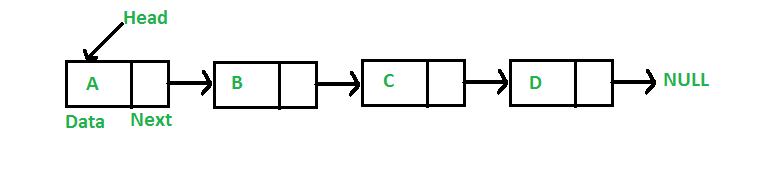
\includegraphics[width=0.7\textwidth]{img/Linkedlist.png}
    \caption{Linked List(\href{https://www.geeksforgeeks.org/data-structures/linked-list/}{Source})}
  \end{figure}
\end{frame}

\begin{frame}[fragile]{Implementation}
\begin{lstlisting}[language=python]
  class LinkedList:
    def __init__(self):
      self.data=None
      self.next=None
    def insert(self,data):
      if self.data==None:
        self.data=data
        self.next=LinkedList()
      else:
        self.next.insert(data)
    def find(self,data):
      if self.data==data:
        return True
      elif self.data==None:
        return False
      else:
        return self.next.find(data)
\end{lstlisting}
\end{frame}

\begin{frame}{Pros and Cons of Linked List}
  \begin{itemize}
    \item Pros:
    \begin{itemize}
      \item Fast to insert: In practice we have more complicated implementation to allow direct jump to the end and insert
      \item memory efficient: memory usage proportion to data stored without special care
      \item easy to remove, rearrange elements
    \end{itemize}
    \item Cons:
    \begin{itemize}
      \item searching is still slow
      \item slow to access data by position
    \end{itemize}
    \item Usage:
    \begin{itemize}
      \item Not particularly useful alone
      \item Usually use as base of other structure
      \item useful when frequently update data but have very few query
    \end{itemize}
  \end{itemize}
\end{frame}
\end{document}
